\section{Optimal Control of Pitch/Travel and Elevation with and without Feedback}\label{sec:10.4}

Previously this report has only been focusing on optimal control of pitch and travel, calculating an optimal trajectory without considering elevation. This will be done in this section. In addition, nonlinear constraints are also added to the optimization problem. 

\subsection{Continous state space form}

By adding elevation $e$ and elevation rate $\dot{e}$ to the state vector, the model can be written on continuous state space form

\begin{equation}
\begin{aligned}
$$\dot{x} = {A_c}x + {B_c}u$$      
\end{aligned}
\end{equation}

where $x = \left[ {\begin{array}{*{20}{r}}\lambda &r&p&{\dot{p}}&e&{\dot{e}} \end{array}}\right]^\top$ and $u = [ {\begin{array}{*{20}{c}}p_c&u_c\end{array}}]^\top$. The system matrices $A_c$ and $B_c$ are given by

\begin{equation}
\begin{aligned}
    $$A_c = \left[ {\begin{array}{*{20}{c}}
0&1&0&0&0&0\\
0&0&{ - {K_2}}&0&0&0\\
0&0&0&1&0&0\\
0&0&{ - {K_1}{K_{pp}}}&{ - {K_1}{K_{dp}}}&0&0\\
0&0&0&0&0&1\\
0&0&0&0&{ - {K_3}{K_{ep}}}&{ - {K_3}{K_{ed}}}
\end{array}} \right]$$
\end{aligned}
\end{equation}


\begin{equation}
\begin{aligned}
$$B_c = \left[ {\begin{array}{*{20}{c}}
0&0\\
0&0\\
0&0\\
{{K_1}{K_{pp}}}&0\\
0&0\\
0&{{K_3}{K_{ep}}}
\end{array}} \right]$$
\end{aligned}
\end{equation}

\subsection{Discretized State Space Model}

The model is discretized by using the Forward Euler Method as in Section \ref{sec:10.2}, given by Equation \ref{eq:forwardeuler}.
Thus, the model can be written on discrete time state space form

\begin{equation}
\begin{aligned}
$${x_{k + 1}} = A{x_k} + B{u_k}$$
\end{aligned}
\end{equation}

where $A$ and $B$ are given by

\begin{equation}
$$A = I + \Delta t{A_c}=\left[ {\begin{array}{*{20}{r}}
  1&\Delta t&0&0&0&0 \\ 
  0&1&{ - \Delta t{K_2}}&0&0&0 \\ 
  0&0&1&h&0&0 \\ 
  0&0&{ - \Delta t{K_1}{K_{pp}}}&{1 - \Delta t{K_l}{K_{dp}}}&0&0 \\ 
  0&0&0&0&1&\Delta t \\ 
  0&0&0&0&{ - \Delta t{K_3}{K_{ep}}}&{1 - \Delta t{K_3}{K_{ed}}} 
\end{array}} \right]$$
\end{equation}\\

\begin{equation}
\begin{aligned}
$$B = \Delta t{B_c} = \left[ {\begin{array}{*{20}{r}}
  0&0 \\ 
  0&0 \\ 
  0&0 \\ 
  {\Delta t{K_1}{K_{pp}}}&0 \\ 
  0&0 \\ 
  0&{\Delta t{K_3}{K_{ep}}} 
\end{array}} \right]$$
\end{aligned}
\end{equation}



\subsection{Optimization problem with new nonlinear constriants}

In this section, as the previous, the objective is to calculate an optimal trajectory from 
${x_0}=[{\lambda_0}\quad 0\quad 0\quad 0 \quad 0\quad 0]^\top$ to 
${x_f}=[{\lambda_f}\quad 0\quad 0\quad 0 \quad 0\quad 0]^\top$

This trajectory is calculated by minimizing the objective function
\begin{equation}
\begin{aligned}
$$\phi  = \sum\limits_{i = 1}^N {{{({\lambda _i} - {\lambda _f})}^2} + {q_1}p_{ci}^2 + {q_2}e_{ci}^2} $$
\end{aligned}
\end{equation}

which is a quadratic objective function that can be reformulated by using equation (4.11) from \cite{Foss2016},
\begin{equation}
\begin{aligned}
$$\phi  = \sum\limits_{i = 0}^{N-1} {(x_{i+1}-x_{i+1}^{ref})^\top Q(x_{i+1}-x_{i+1}^{ref}) + u_t^\top Ru_t} $$
\end{aligned}
\end{equation}

where 

$$Q = \left[ {\begin{array}{*{20}{c}}
  1&0&0&0&0&0 \\ 
  0&0&0&0&0&0 \\ 
  0&0&0&0&0&0 \\ 
  0&0&0&0&0&0 \\ 
  0&0&0&0&0&0 \\ 
  0&0&0&0&0&0 
\end{array}} \right],R = \left[ {\begin{array}{*{20}{c}}
  {{q_1}}&0 \\ 
  0&{{q_2}} 
\end{array}} \right]$$

In addition to the equality constraints from previous sections, a nonlinear inequality constraint is added on the elevation. To calculate this nonlinear inequality constraint, a function in MATLAB is created and added in the built-in function for calculating the optimal trajectory. The nonlinear inequality constraint added is

\begin{equation}
\begin{aligned}
$${e_k} \ge \alpha \exp ( - \beta {({\lambda _k} - {\lambda _t})^2}) \quad  \forall k \in \{ 1,...,N\} $$
\end{aligned}
\end{equation}

which in order to be implemented in the built-in function is reformulated as
\begin{equation}
\begin{aligned}
$$c({x_k}) = \alpha \exp ( - \beta {({\lambda _k} - {\lambda _t})^2}) - {e_k} \le 0$$
\end{aligned}
\end{equation}

with $\alpha = 0.2$, $\beta = 20$ and $\lambda_k = \frac{2\pi}{3}$.
Both of these functions are passed into the MATLAB-function \texttt{fmincon}, which calculates the optimal trajectory for the helicopter. $\Delta t = 0.25 $ and $N = 40$ are used, which yields an optimizing horizon of 10 seconds.

With the equality constraints from previous sections and the new nonlinear constraint, the optimization problem can be stated as

\begin{subequations}
    \begin{equation}
    \begin{aligned}
        $$\mathop {\min }\limits_z  = {z^\top}Gz$$
    \end{aligned}
    \end{equation}
    subject to
        \begin{equation}
    \begin{aligned}
        $$ A$_{eq}$z = b$_{eq}$ $$
    \end{aligned}
    \end{equation}
    \begin{equation}
    \begin{aligned}
        $$c({x_k}) \le 0$$
    \end{aligned}
    \end{equation}
    \begin{equation}
    \begin{aligned}
        $$p_{min} \le p_k \le p_{max}$$
    \end{aligned}
    \end{equation}
\end{subequations}

It is worth noting that the default optimizing algorithm in MATLAB did not converge to an optimal solution. It was therefore necessary to use the SQP (Sequential Quadratic Programming) algorithm to solve the optimization problem.

\subsection{Compare results with and without feedback}\label{subsec:feedback}

The optimal input sequence calculated using the new cost function and constraints is implemented in Simulink, first simulated without using feedback. For simulation with feedback, the LQR is implemented as in subsection~\ref{subsec:lqr} and now with all the states connected,

$${Q_{lqr}} = \left[ {\begin{array}{*{20}{c}}
  1&0&0&0&0&0 \\ 
  0&1&0&0&0&0 \\ 
  0&0&1&0&0&0 \\ 
  0&0&0&1&0&0 \\ 
  0&0&0&0&1&0 \\ 
  0&0&0&0&0&1 
\end{array}} \right],{R_{lqr}} = \left[ {\begin{array}{*{20}{c}}
  1&0 \\ 
  0&1 
\end{array}} \right]$$

Different values for $Q_{lqr}$ and $R_{lqr}$ are experimented with to obtain a more smooth and even trajectory for the helicopter. 

\subsubsection{Decoupled states}
In this model, the elevation $e$ and elevation rate $\dot{e}$ is completely decoupled from the other states. This does not fit well with reality. At small pitch angles, elevation is mostly dependent on pitch, but at larger pitch angles the travel rate and elevation rate is dependent variables. This simplification of the model yields an offset in the solution. Coupling all the states together would provide a more precise, but also a more complex model.

\subsection{Optional: More constraints}\label{subsec:constraints}

With the optimal trajectory calculated by minimizing the objective function, the helicopter went slightly beyond $\lambda_f = \pi$ before it turned back and stabilized at $\lambda_f$. Hence, it was tempting to try adding other constraints on the objective function. Constraining the elevation rate $\dot{e}$, and velocity (travel rate) $\dot{\lambda}$, should produce a different result that may prevent the overshoot.
\begin{table}[H]
\centering
\label{constraints}
\renewcommand{\arraystretch}{1.1}
\caption{Additional constraints}
\begin{tabular}{lll}
\toprule
Constraint    &    $\dot{\lambda}$        & $\dot{e}$ \\
\midrule
1             & $\frac{-20\pi}{180} - \frac{5\pi}{180}$  & $\frac{-\pi}{180} - 0$                   \\
2             & $\frac{-5\pi}{180} - \frac{5\pi}{180}$ & $\frac{-\pi}{180} - \frac{10\pi}{180}$   \\
3             & $\frac{-5\pi}{180} - \frac{5\pi}{180}$ & $\frac{-\pi}{180} - \frac{10\pi}{180}$   \\
4             & $\frac{-10\pi}{180} - \frac{10\pi}{180}$ & $\frac{-5\pi}{180} - \frac{5\pi}{180}$   \\
5             & - & -   \\
\bottomrule
\end{tabular}
\end{table}

Very strict constraints on the objective function results in the SQP-algorithm not converging to an optimal solution. It was therefore necessary to loosen the constraints. All the constraints, except the third, were simulated with 40 time steps. The third constraint were simulated using 80 time steps. 

\subsection{Results and discussion}
This subsection will present and discuss the results from the previous subsections.
\subsubsection{Without feedback}
The optimal trajectory calculated using the new objective function and nonlinear constraints was first simulated without feedback.

\begin{figure}[H]
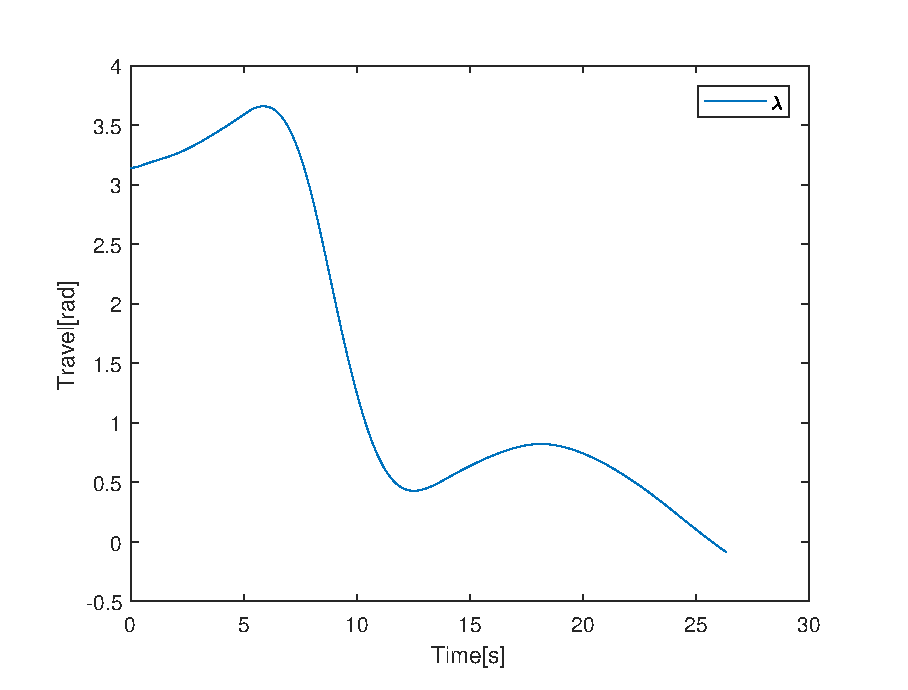
\includegraphics[width=1\linewidth, height=7cm]{data_10.4/travel_uten_feedback_eps.eps} 
\centering
\caption{Observed travel without feedback}\label{fig:travelufeedback}
\end{figure}

\begin{figure}[H]
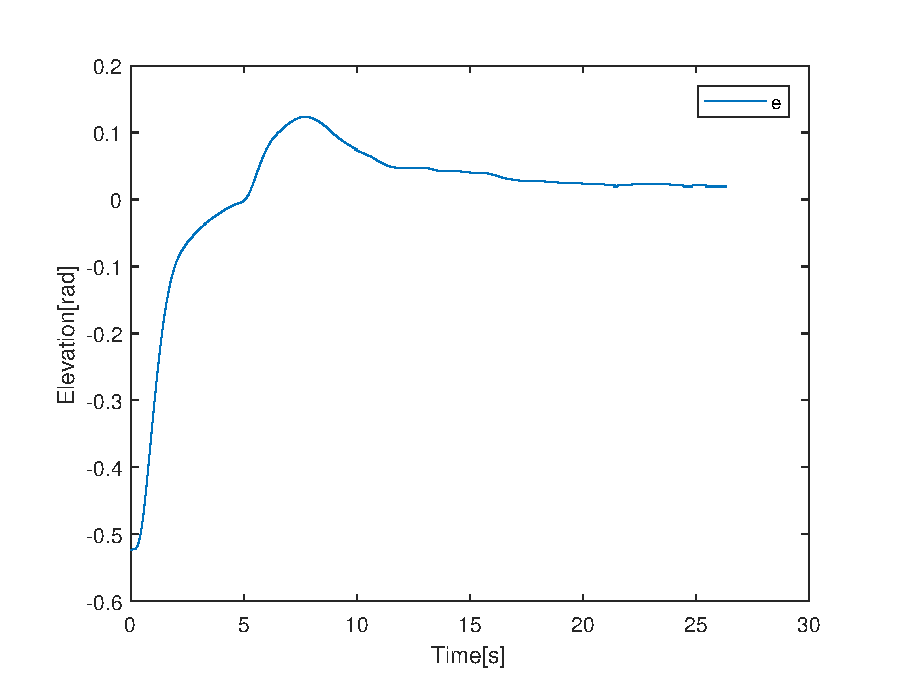
\includegraphics[width=1\linewidth, height=7cm]{data_10.4/elevation_uten_feedback_eps.eps} 
\centering
\caption{Observed elevation without feedback}\label{fig:elevationufeedback}
\end{figure}

Figure~\ref{fig:travelufeedback} and Figure~\ref{fig:elevationufeedback} shows the helicopters trajectory when simulating without feedback. The helicopter drifted away from the start point which lead to the helicopter not stopping at $\lambda = 0$. After 15 seconds the output was set to zero, which explains why the helicopter drifted away from the desired position. There were no significant differences on the observed elevation with and without feedback. As shown in figure~\ref{fig:elevationufeedback}, the observed elevation does not differ much from the optimization. 

\subsubsection{With feedback}

Feedback was again implemented as presented in subsection~\ref{subsec:feedback}. The feedback gain matrix $K$ was adjusted by changing the weights in the $Q_{lqr}$ and $R_{lqr}$ matrix. 

\begin{figure}[H]
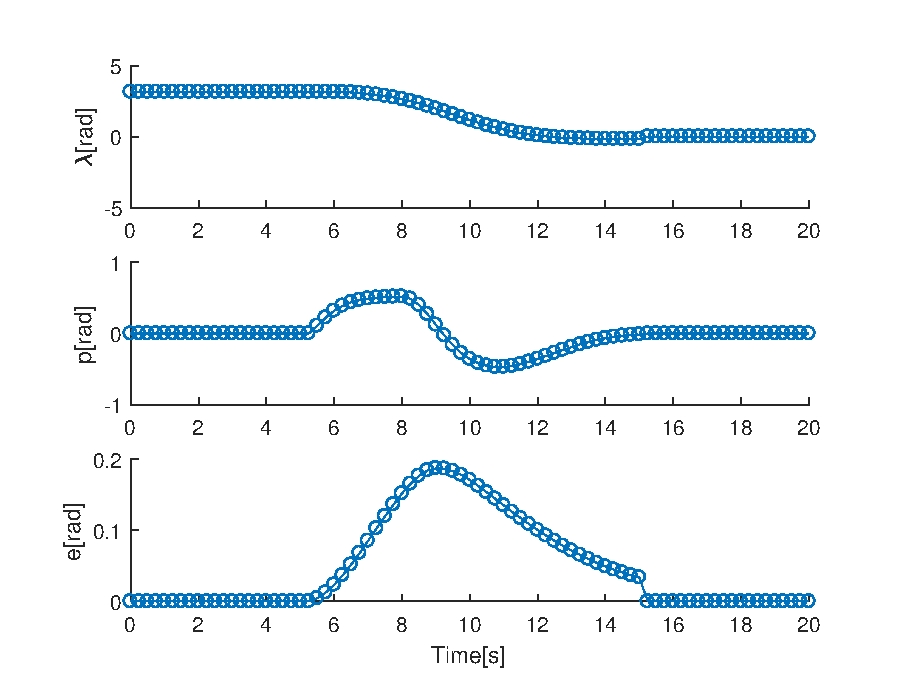
\includegraphics[width=1\linewidth, height=8cm]{data_10.4/states_eps.eps} 
\centering
\caption{The calculated optimal trajectory showing travel, $\lambda$, pitch, $p$, and elevation, $e$.}\label{fig:states_1}
\end{figure}

Figure~\ref{fig:states_1} shows the calculated optimal trajectory for travel $\lambda$, pitch $p$, and elevation $e$. In comparison with   Section~\ref{sec:10.3}, the introduction of the two new states and the nonlinear constraint on elevation is clearly visible as the elevation now has a distinct trajectory. 

\begin{figure}[H]
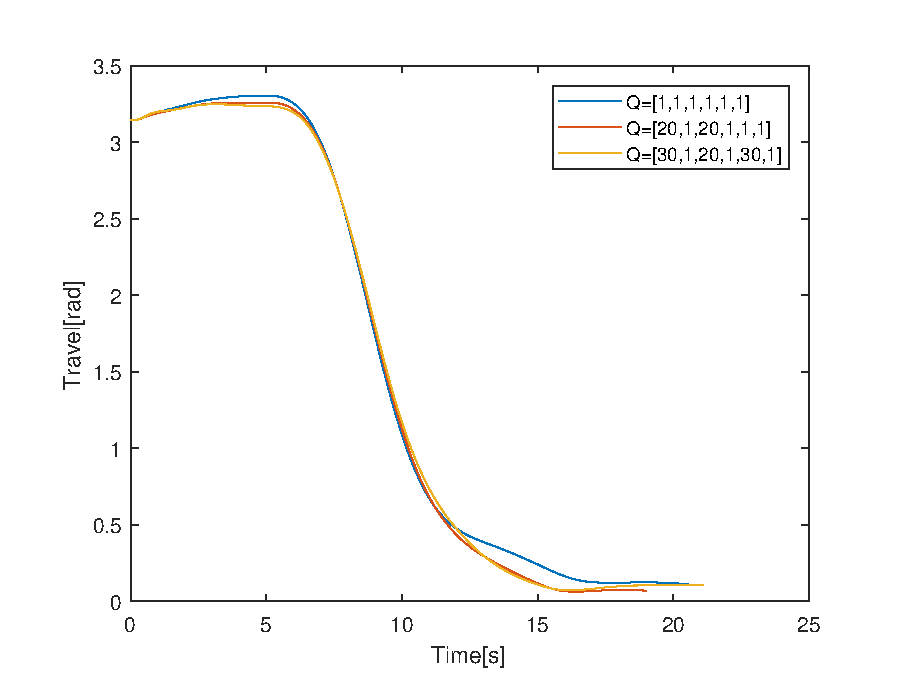
\includegraphics[width=1\linewidth, height=8cm]{data_10.4/travel_eps.eps} 
\centering
\caption{Observed travel with three different Q matrices}\label{fig:travel1}
\end{figure}

\begin{figure}[H]
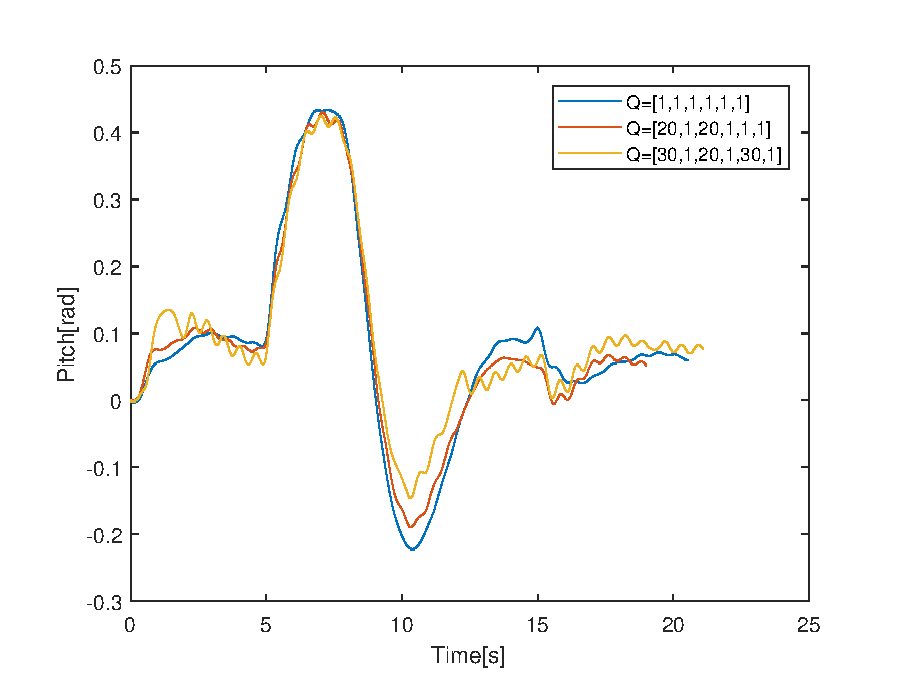
\includegraphics[width=1\linewidth, height=8cm]{data_10.4/pitch_eps.eps} 
\centering
\caption{Observed pitch with three different Q matrices}\label{fig:pitch1}
\end{figure}

\begin{figure}[H]
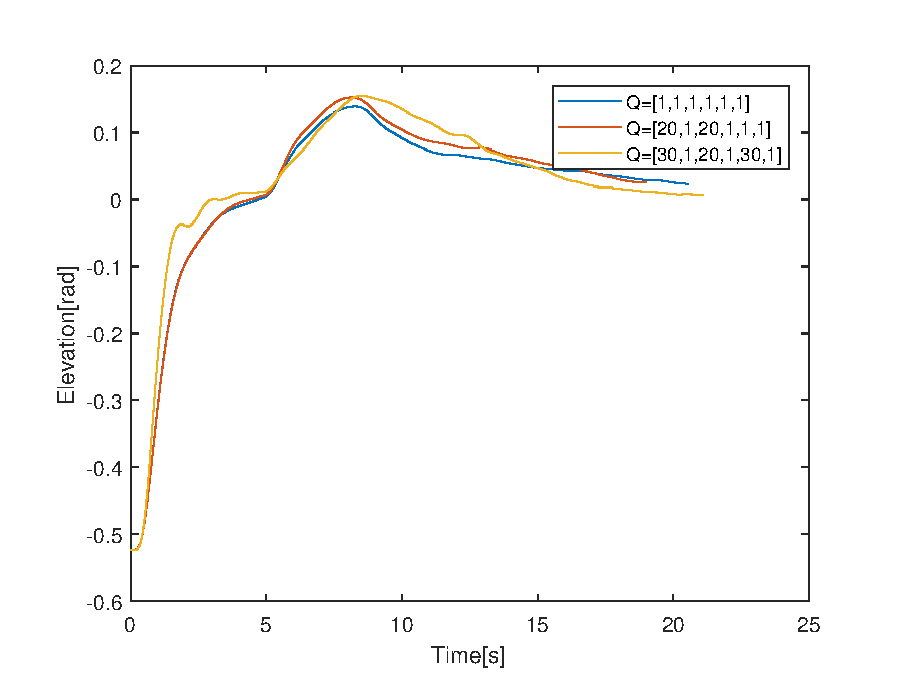
\includegraphics[width=1\linewidth, height=8cm]{data_10.4/elevation_eps.eps} 
\centering
\caption{Observed elevation with three different Q matrices}\label{fig:elevation1}
\end{figure}

Figure~\ref{fig:travel1}, ~\ref{fig:pitch1} and ~\ref{fig:elevation1} shows how the helicopter performs with respect to travel, pitch and elevation. In each graph, the $K$ matrix was calculated using three different Q matrices, where the diagonals were $[\begin{matrix}
   1 & 1 & 1 & 1 & 1 & 1\end{matrix}]$, $[\begin{matrix}
   20 & 1 & 20 & 1 & 1 & 1\end{matrix}]$ and $[\begin{matrix}
   30 & 1 & 20 & 1 & 30 & 1\end{matrix}]$ with the diagonal of $R$ being $[\begin{matrix}1 & 1\end{matrix}]$ for all three Q matrices. 
It is evident, as expected, that the weighing on the different states has an impact on how the helicopter behaves, but it does not have a significant impact on the observed travel. The resulting travel from the three different cases does not differ much, there is some differences in the time to convergence, but all three follow a similar trajectory. 
In regard to pitch, increased weights introduced more small oscillations, but it also decreased the larger oscillations. Neglecting the small oscillations, the pitch is very similar to the calculated pitch in figure~\ref{fig:states_1}.
The observed elevation for the three different cases is, as for the travel, no significant difference compared to the optimization. The second case has a slightly lower decrease in elevation.

\subsubsection{Additional constraints}
In order to study the affect of constraining different states, constraints as described in \ref{subsec:constraints} were introduced to the optimization problem.

\begin{figure}[H]
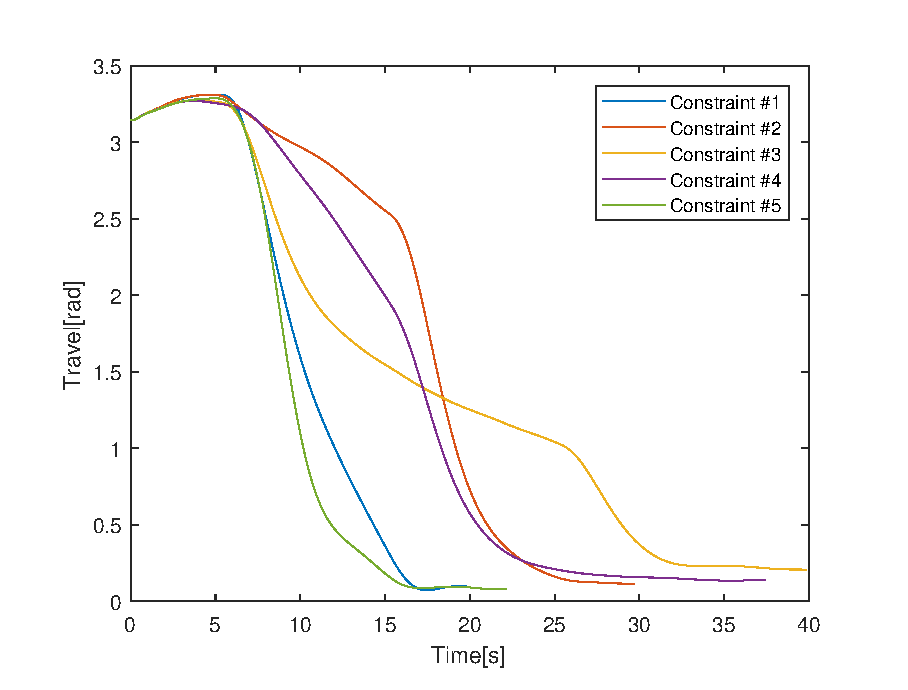
\includegraphics[width=1\linewidth, height=8cm]{data_10.4/constraints_eps.eps} 
\centering
\caption{Observed travel with five different constraints as described in \ref{subsec:constraints}}\label{fig:ctravel}
\end{figure}

The observed travel for the five different constraints displays a good representation of the high consequence of strict constraints. The first and fifth constraint are fairly similar, except slight difference at the end of simulation. The second, third and fourth constraint are significantly slower than the two other. The second and third (which was simulated with 80 time steps) constraint did not converge to an optimal solution, and the simulation of the two displayed an odd behaviour with respect to travel rate. This is observable in figure~\ref{fig:ctravel} after about 20 and 30 seconds respectively. 

\begin{figure}[H]
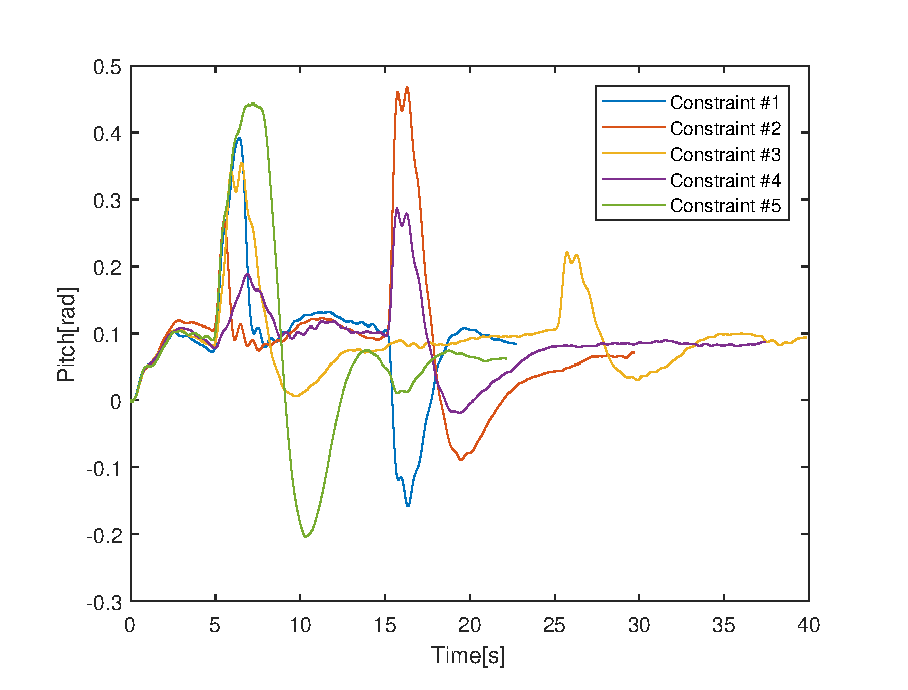
\includegraphics[width=1\linewidth, height=8cm]{data_10.4/constraints_p_eps.eps} 
\centering
\caption{Observed pitch with constraints}\label{fig:cpitch}
\end{figure}

With the new constraints there was a big difference in the observed pitch for the five cases. Compared to the observed travel, they correspond well to how the helicopter behaved, where high differences in pitch leads to high travel rate. 

\begin{figure}[H]
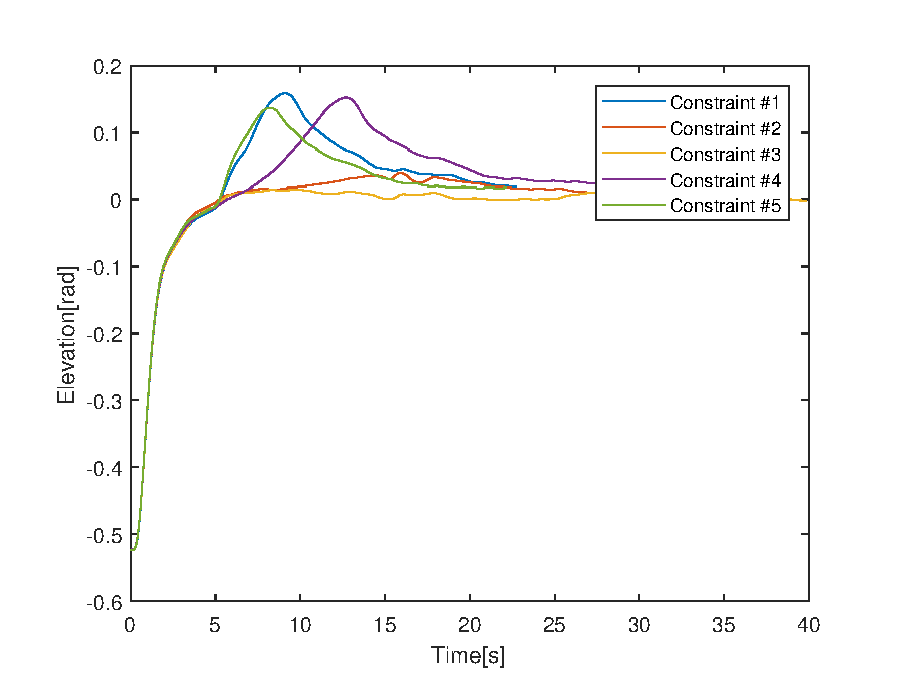
\includegraphics[width=1\linewidth, height=8cm]{data_10.4/constraints_e_eps.eps} 
\centering
\caption{Observed elevation with constraints}\label{fig:celev}
\end{figure}

For the first three cases the observed elevation is very similar, as expected with the strict constraints on elevation rate. The fourth constraint, where the elevation rate had more room to manoeuvre in, yielded a similar behaviour as previous simulations. 

\subsubsection{Discussion}
With the introduction of elevation to the system states, the optimization problem now included a new dimension, elevation. In section~\ref{sec:10.3} the helicopter had a nearly constant elevation, where the optimization problem focused on the first four states. With the elevation included, the helicopter now behaved more naturally, neglecting the unrealistic decoupled states, with an the elevation being dependent on pitch and travel rate.

For the simulation without feedback, the helicopter behaved as expected, with a slight overshoot, before drifting away from the desired $\lambda$ value. The observed elevation was very similar to the calculated elevation. The behaviour of the helicopter may be improved with a better tuning of the regulators, but as this was not the scope of this report we did not prioritize this.

With feedback and LQR implemented again, a series of different weights on the $Q_{lqr}$ and $R_{lqr}$ were tested. As presented, the resulting travel, pitch and elevation did not differ much. We expected a bigger difference in the behaviour, especially with respect to travel and pitch. The LQR corrects the trajectory and does not let the helicopter deviate much from the calculated optimal trajectory. The three cases in figure~\ref{fig:travel1}, ~\ref{fig:pitch1} and ~\ref{fig:elevation1} does not differ much from the calculated trajectory presented in figure~\ref{fig:states_1}. It is also worth noting that we experienced some technical problems with the QuaRC encoder during these tests, as was reported to the learning assistants. These problems, which were present occasionally, may have influenced the results. 
The additional constraints clearly showed the huge difference strict constraints have on the optimization problem. The four additional constraints added were not meant to give a "better" performance, but to give a brief overview of how the constraints affect the solution to the problem. With very strict constraints as in constraint two and three, the algorithm did not converge to an optimal solution. This was clearly visible in figure~\ref{fig:ctravel}, as constraint two and three had an odd travel at the end of simulation. With a more defined task, these additional constraints may provide a behaviour that is more satisfying.